\documentclass{standalone}
\usepackage{tikz}
\usetikzlibrary{patterns, positioning}
\usepackage[sfdefault]{ClearSans} %% option 'sfdefault' activates Clear Sans as the default text font
\usepackage[T1]{fontenc}

\begin{document}
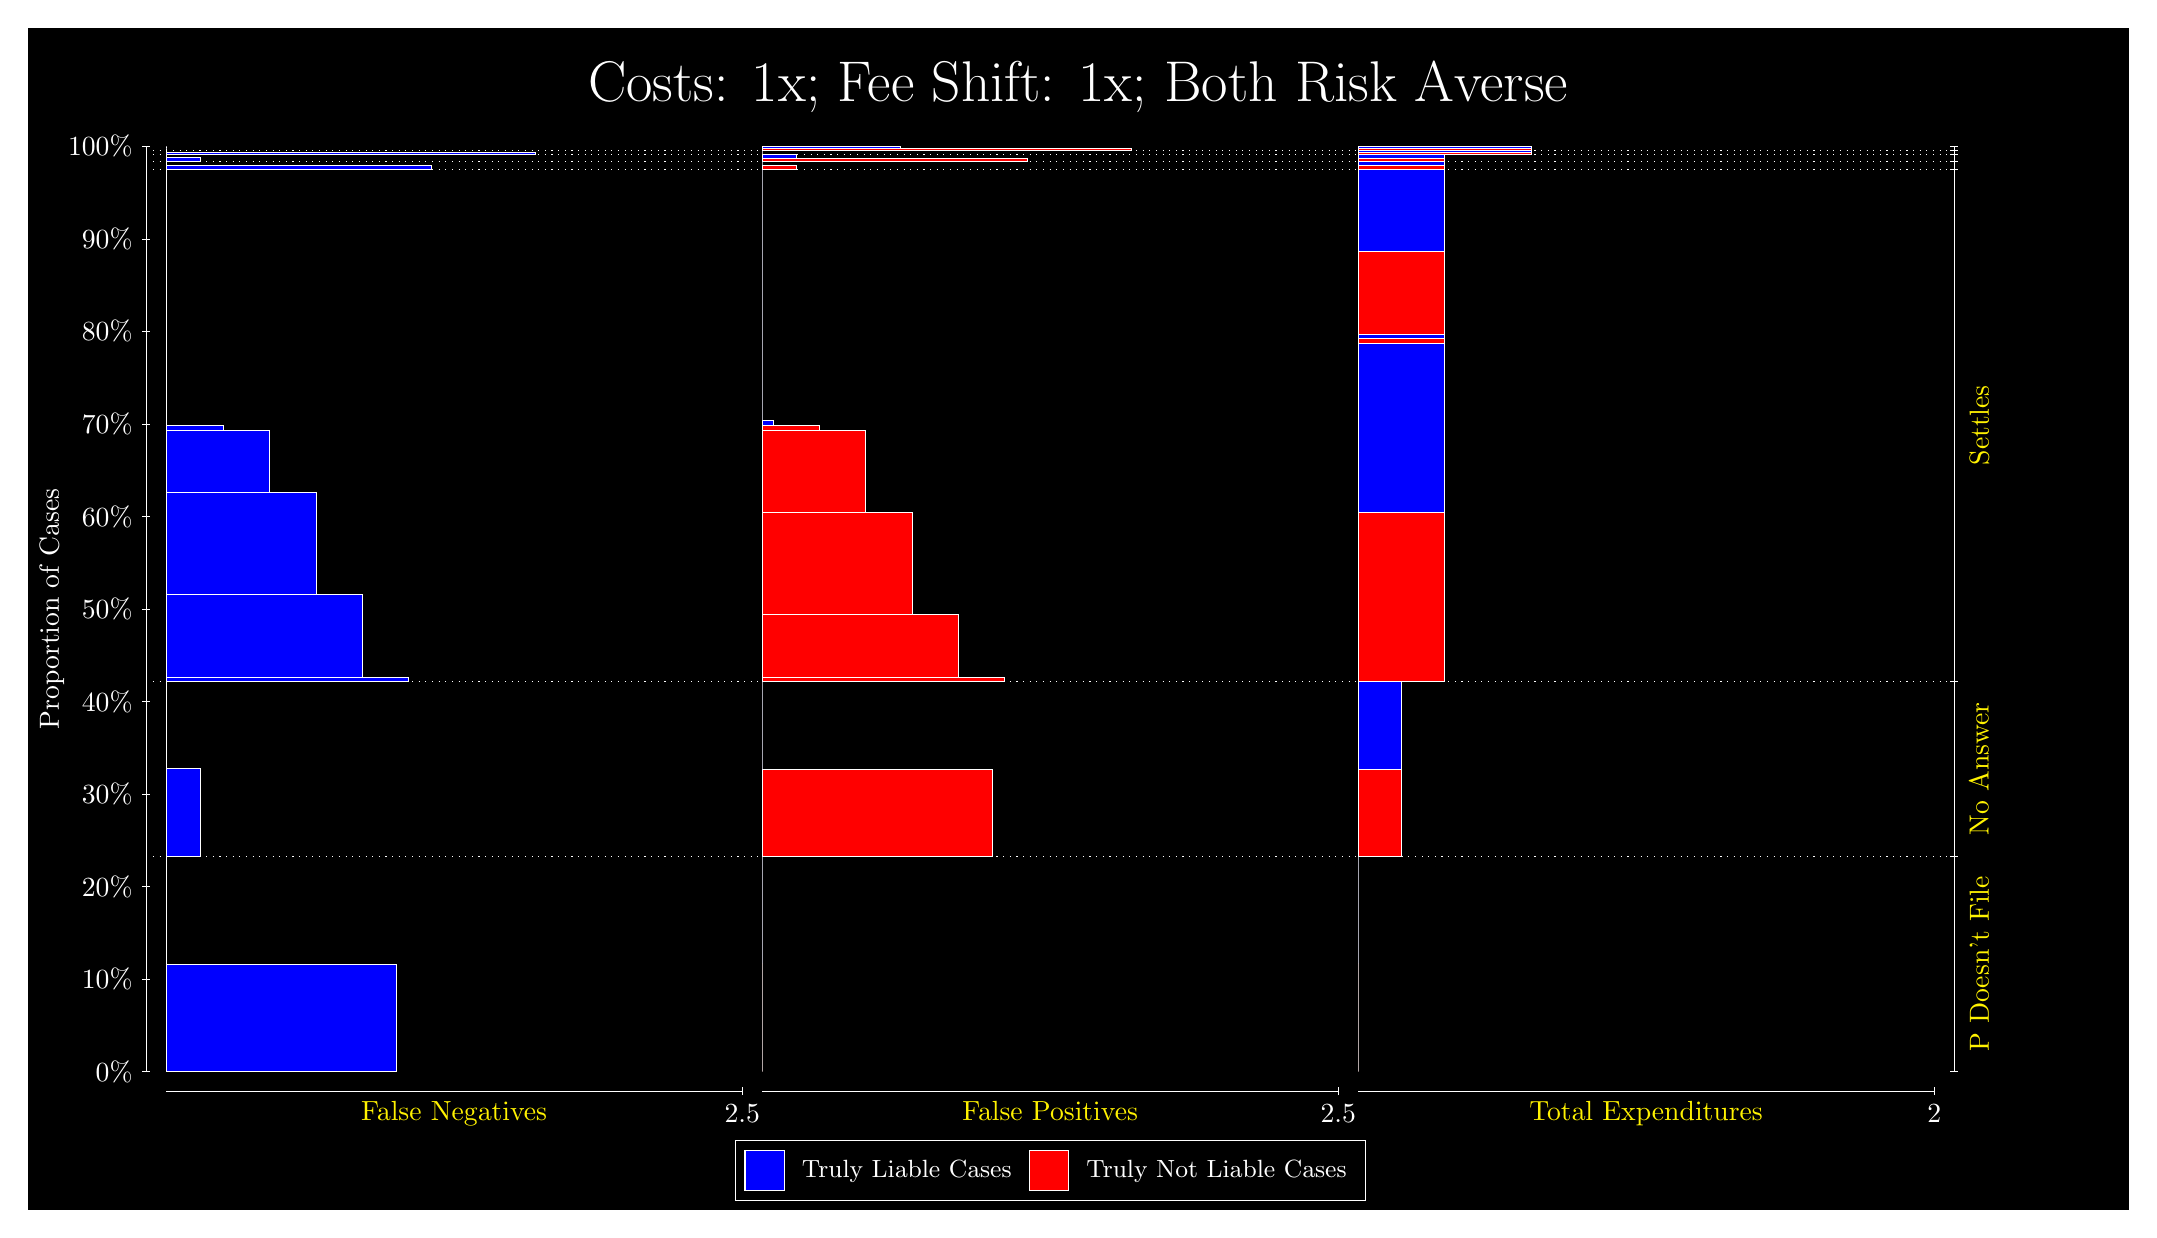
\begin{tikzpicture}
\draw[fill=black] (0,0) rectangle (26.667,15);
\draw[text=white] (0,13.5) rectangle (26.667,15) node[midway] {\huge Costs: 1x; Fee Shift: 1x; Both Risk Averse};
\draw[white, very thin] (1.5,1.75) -- (1.5,13.5);
\node[rotate=90, text=white, anchor=center] at (0.3, 7.625) {Proportion of Cases};
\draw[white, very thin] (1.45,1.75) -- (1.55,1.75);
\node[text=white, anchor=east] at (1.45, 1.75) {0\%};
\draw[white, very thin] (1.45,2.925) -- (1.55,2.925);
\node[text=white, anchor=east] at (1.45, 2.925) {10\%};
\draw[white, very thin] (1.45,4.1) -- (1.55,4.1);
\node[text=white, anchor=east] at (1.45, 4.1) {20\%};
\draw[white, very thin] (1.45,5.275) -- (1.55,5.275);
\node[text=white, anchor=east] at (1.45, 5.275) {30\%};
\draw[white, very thin] (1.45,6.45) -- (1.55,6.45);
\node[text=white, anchor=east] at (1.45, 6.45) {40\%};
\draw[white, very thin] (1.45,7.625) -- (1.55,7.625);
\node[text=white, anchor=east] at (1.45, 7.625) {50\%};
\draw[white, very thin] (1.45,8.8) -- (1.55,8.8);
\node[text=white, anchor=east] at (1.45, 8.8) {60\%};
\draw[white, very thin] (1.45,9.975) -- (1.55,9.975);
\node[text=white, anchor=east] at (1.45, 9.975) {70\%};
\draw[white, very thin] (1.45,11.15) -- (1.55,11.15);
\node[text=white, anchor=east] at (1.45, 11.15) {80\%};
\draw[white, very thin] (1.45,12.325) -- (1.55,12.325);
\node[text=white, anchor=east] at (1.45, 12.325) {90\%};
\draw[white, very thin] (1.45,13.5) -- (1.55,13.5);
\node[text=white, anchor=east] at (1.45, 13.5) {100\%};

\draw[white, very thin] (24.457,1.75) -- (24.457,13.5);
\draw[white, very thin] (24.407,1.75) -- (24.507,1.75);
\node[anchor=west] at (24.407, 1.75) {};
\draw[white, very thin] (24.407,4.4824) -- (24.507,4.4824);
\node[anchor=west] at (24.407, 4.4824) {};
\draw[white, very thin] (24.407,6.7038) -- (24.507,6.7038);
\node[anchor=west] at (24.407, 6.7038) {};
\draw[white, very thin] (24.407,13.211) -- (24.507,13.211);
\node[anchor=west] at (24.407, 13.211) {};
\draw[white, very thin] (24.407,13.304) -- (24.507,13.304);
\node[anchor=west] at (24.407, 13.304) {};
\draw[white, very thin] (24.407,13.398) -- (24.507,13.398);
\node[anchor=west] at (24.407, 13.398) {};
\draw[white, very thin] (24.407,13.449) -- (24.507,13.449);
\node[anchor=west] at (24.407, 13.449) {};
\draw[white, very thin] (24.407,13.5) -- (24.507,13.5);
\node[anchor=west] at (24.407, 13.5) {};

\draw[white, very thin, fill=blue] (1.75,1.75) rectangle (4.6775,3.107);
\draw[white, very thin, fill=red] (1.75,3.107) rectangle (1.75,4.4824);
\draw[white, very thin, fill=blue] (1.75,4.4824) rectangle (2.1891,5.6023);
\draw[white, very thin, fill=red] (1.75,5.6023) rectangle (1.75,6.7038);
\draw[white, very thin, fill=blue] (1.75,6.7038) rectangle (4.8239,6.7609);
\draw[white, very thin, fill=blue] (1.75,6.7609) rectangle (4.2384,7.8101);
\draw[white, very thin, fill=blue] (1.75,7.8101) rectangle (3.6529,9.1075);
\draw[white, very thin, fill=blue] (1.75,9.1075) rectangle (3.0674,9.8956);
\draw[white, very thin, fill=blue] (1.75,9.8956) rectangle (2.4819,9.9574);
\draw[white, very thin, fill=red] (1.75,9.9574) rectangle (1.75,13.211);
\draw[white, very thin, fill=blue] (1.75,13.211) rectangle (5.1167,13.253);
\draw[white, very thin, fill=red] (1.75,13.253) rectangle (1.75,13.304);
\draw[white, very thin, fill=blue] (1.75,13.304) rectangle (2.1891,13.356);
\draw[white, very thin, fill=red] (1.75,13.356) rectangle (1.75,13.398);
\draw[white, very thin, fill=blue] (1.75,13.398) rectangle (6.4341,13.421);
\draw[white, very thin, fill=red] (1.75,13.421) rectangle (1.75,13.449);
\draw[white, very thin, fill=red] (1.75,13.449) rectangle (1.75,13.472);
\draw[white, very thin, fill=blue] (1.75,13.472) rectangle (1.75,13.5);
\draw[white, very thin, fill=red] (9.3189,1.75) rectangle (9.3189,3.1253);
\draw[white, very thin, fill=blue] (9.3189,3.1253) rectangle (9.3189,4.4824);
\draw[white, very thin, fill=red] (9.3189,4.4824) rectangle (12.246,5.584);
\draw[white, very thin, fill=blue] (9.3189,5.584) rectangle (9.3189,6.7038);
\draw[white, very thin, fill=red] (9.3189,6.7038) rectangle (12.393,6.7609);
\draw[white, very thin, fill=red] (9.3189,6.7609) rectangle (11.807,7.5547);
\draw[white, very thin, fill=red] (9.3189,7.5547) rectangle (11.222,8.852);
\draw[white, very thin, fill=red] (9.3189,8.852) rectangle (10.636,9.8956);
\draw[white, very thin, fill=red] (9.3189,9.8956) rectangle (10.051,9.9574);
\draw[white, very thin, fill=blue] (9.3189,9.9574) rectangle (9.4652,10.019);
\draw[white, very thin, fill=blue] (9.3189,10.019) rectangle (9.3189,13.211);
\draw[white, very thin, fill=red] (9.3189,13.211) rectangle (9.758,13.263);
\draw[white, very thin, fill=blue] (9.3189,13.263) rectangle (9.3189,13.304);
\draw[white, very thin, fill=red] (9.3189,13.304) rectangle (12.686,13.346);
\draw[white, very thin, fill=blue] (9.3189,13.346) rectangle (9.758,13.398);
\draw[white, very thin, fill=red] (9.3189,13.398) rectangle (9.3189,13.425);
\draw[white, very thin, fill=blue] (9.3189,13.425) rectangle (9.3189,13.449);
\draw[white, very thin, fill=red] (9.3189,13.449) rectangle (14.003,13.472);
\draw[white, very thin, fill=blue] (9.3189,13.472) rectangle (11.075,13.5);
\draw[white, very thin, fill=red] (16.888,1.75) rectangle (16.888,3.1253);
\draw[white, very thin, fill=blue] (16.888,3.1253) rectangle (16.888,4.4824);
\draw[white, very thin, fill=red] (16.888,4.4824) rectangle (17.437,5.584);
\draw[white, very thin, fill=blue] (16.888,5.584) rectangle (17.437,6.7038);
\draw[white, very thin, fill=red] (16.888,6.7038) rectangle (17.986,8.852);
\draw[white, very thin, fill=blue] (16.888,8.852) rectangle (17.986,10.999);
\draw[white, very thin, fill=red] (16.888,10.999) rectangle (17.986,11.061);
\draw[white, very thin, fill=blue] (16.888,11.061) rectangle (17.986,11.118);
\draw[white, very thin, fill=red] (16.888,11.118) rectangle (17.986,12.162);
\draw[white, very thin, fill=blue] (16.888,12.162) rectangle (17.986,13.211);
\draw[white, very thin, fill=red] (16.888,13.211) rectangle (17.986,13.263);
\draw[white, very thin, fill=blue] (16.888,13.263) rectangle (17.986,13.304);
\draw[white, very thin, fill=red] (16.888,13.304) rectangle (17.986,13.346);
\draw[white, very thin, fill=blue] (16.888,13.346) rectangle (17.986,13.398);
\draw[white, very thin, fill=red] (16.888,13.398) rectangle (19.083,13.425);
\draw[white, very thin, fill=blue] (16.888,13.425) rectangle (19.083,13.449);
\draw[white, very thin, fill=red] (16.888,13.449) rectangle (19.083,13.472);
\draw[white, very thin, fill=blue] (16.888,13.472) rectangle (19.083,13.5);
\draw[white, dotted] (1.5,4.4824) -- (24.457,4.4824);
\draw[white, dotted] (1.5,6.7038) -- (24.457,6.7038);
\draw[white, dotted] (1.5,13.211) -- (24.457,13.211);
\draw[white, dotted] (1.5,13.304) -- (24.457,13.304);
\draw[white, dotted] (1.5,13.398) -- (24.457,13.398);
\draw[white, dotted] (1.5,13.449) -- (24.457,13.449);
\draw[white, very thin] (1.75,1.5) -- (9.0689,1.5);
\node[text=yellow, anchor=north] at (5.4094, 1.5) {False Negatives};
\draw[white, very thin] (9.0689,1.45) -- (9.0689,1.55);
\node[text=white, anchor=north] at (9.0689, 1.45) {2.5};

\draw[white, very thin] (9.3189,1.5) -- (16.638,1.5);
\node[text=yellow, anchor=north] at (12.978, 1.5) {False Positives};
\draw[white, very thin] (16.638,1.45) -- (16.638,1.55);
\node[text=white, anchor=north] at (16.638, 1.45) {2.5};

\draw[white, very thin] (16.888,1.5) -- (24.207,1.5);
\node[text=yellow, anchor=north] at (20.547, 1.5) {Total Expenditures};
\draw[white, very thin] (24.207,1.45) -- (24.207,1.55);
\node[text=white, anchor=north] at (24.207, 1.45) {2};

\node[text=yellow, centered, rotate=90] at (24.777, 3.1162) {P Doesn't File};
\node[text=yellow, centered, rotate=90] at (24.777, 5.5931) {No Answer};
\node[text=yellow, centered, rotate=90] at (24.777, 9.9574) {Settles};





\draw (12.978300999999998,1.5) node[draw=none] (baseCoordinate) {};
\begin{scope}[align=center]
        \matrix[scale=0.5, draw=white, below=0.5cm of baseCoordinate, nodes={draw}, column sep=0.1cm]{
            \node[rectangle, draw, minimum width=0.5cm, minimum height=0.5cm, fill=blue] {}; &
            \node[draw=none, font=\small, text=white] (B) {Truly Liable Cases}; &
            \node[rectangle, draw, minimum width=0.5cm, minimum height=0.5cm, fill=red] {}; &
            \node[draw=none, font=\small, text=white] (B) {Truly Not Liable Cases}; \\
            };
\end{scope}

\end{tikzpicture}
\end{document}